%!TEX root = ../template.tex
%%%%%%%%%%%%%%%%%%%%%%%%%%%%%%%%%%%%%%%%%%%%%%%%%%%%%%%%%%%%%%%%%%%%
%% chapter6.tex
%% NOVA thesis document file
%%
%% Chapter with the vision system description.
%%%%%%%%%%%%%%%%%%%%%%%%%%%%%%%%%%%%%%%%%%%%%%%%%%%%%%%%%%%%%%%%%%%%
\chapter{Vision System}
\label{cha:vision_system}

\begin{quotation}
\begin{flushright}
\itshape
«Quotation»\\
\textbf{- Author}
\end{flushright}
\end{quotation}

The vision system is a vital component of the whole system's architecture. On this chapter, a detailed description of this system will be provided. The chapter will start with a general system overview. It will follow with a physical description of the camera, then the camera attachment to the robot, and later, camera calibration. The chapter will end with an overview of the integrations with \gls{ros} and Gazebo.

% ==========================
% = Overview =
% ==========================

\section{Overview}
\label{sec:vision_system_overview}

The vision system is composed by an Intel\textregistered RealSense\texttrademark{} D415 depth camera. It provides not only \gls{rgb} data but also \glsfirst{ir} and depth data.\\

The camera is small, lightweight, low cost, and it is suitable for indoor or outdoor environments. It has high resolution in both \gls{rgb} and depth data, and up to 90 \gls{fps} of frame rate for depth data. It features a range to over 10 \si{\meter}.

It features self-calibration capabilities controlled via its open source \gls{sdk}. The \gls{sdk} has wrappers for several languages and platforms, including \gls{ros}.

% section vision_system_overview

% ==========================
% = Physical Description =
% ==========================

\section{Physical Description}
\label{sec:vision_system_physical_description}

D415 depth camera has a small form factor of $29 \times 20 \times 23$ \si{\milli\meter} (Length $\times$ Depth $\times$ Height). Inside, it has an Intel\textregistered{} RealSense\texttrademark{} Vision Processor D4 and a Depth Module. The vision processor is common among the D400 camera series. The depth module for this camera features an \gls{ir} projector, two stereo cameras and an \gls{rgb} camera (Fig. \ref{fig:camera_physical_description}).\\

The camera has USB-C connector and comes with a USB-C/USB-A cable to connect the camera to a computer. It comes with 3 mounting points, two M3 thread holes on the back of the camera, and one 1/4‑20 UNC thread mounting point on the bottom, not visible on Figure \ref{fig:camera_physical_description}. A tripod stand is also supplied to be assembled on the 1/4-20 UNC mounting point.

\begin{figure}[htbp]
	\centering
	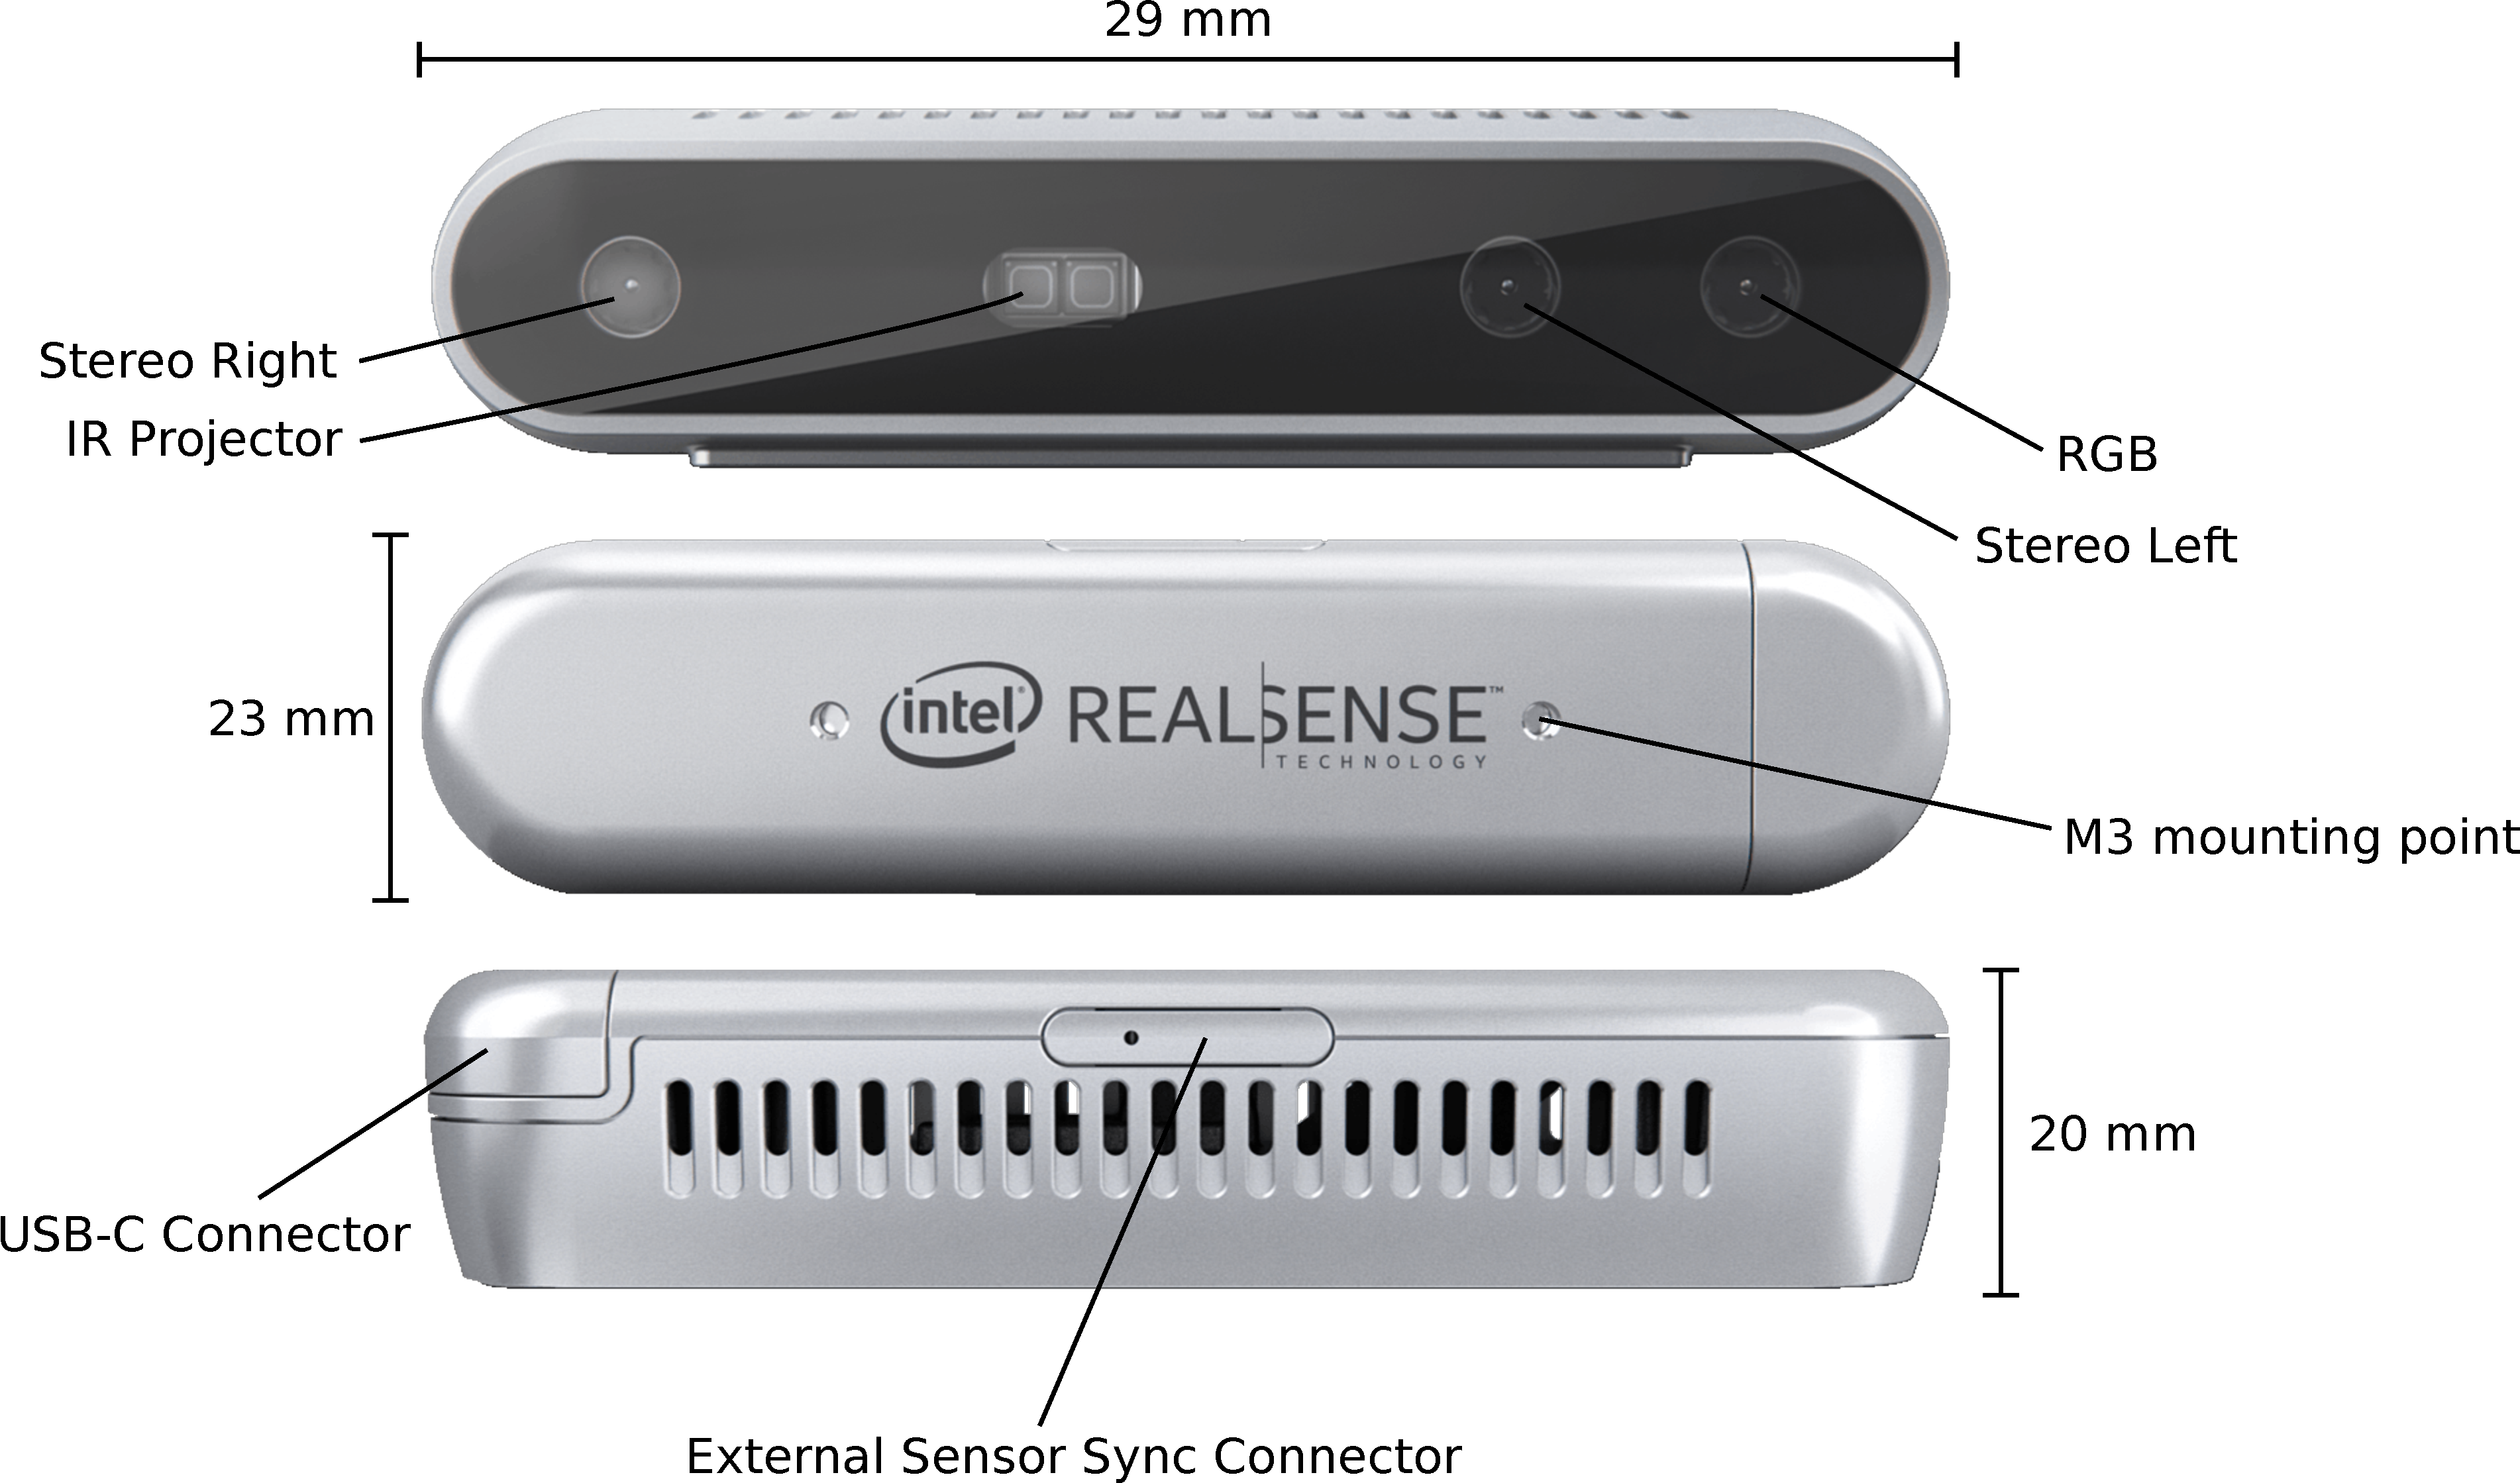
\includegraphics[width=\textwidth]{camera_physical_description}
	\caption{Intel\textregistered{} RealSense\texttrademark{} D415 camera's physical description. Courtesy of Intel\textregistered{} and adapted from \cite{IntelRealSense_depth_camera_d415}.}
	\label{fig:camera_physical_description}
\end{figure}

% section vision_system_physical_description

\section{Camera Attachment to Robot}
\label{sec:vision_system_camera_attachment}

% section vision_system_camera_attachment

\section{Camera Calibration}
\label{sec:vision_system_camera_calibration}

% section vision_system_camera_calibration

% ==========================
% = Integration with ROS =
% ==========================

\section{Integration with \gls{ros}}
\label{sec:vision_system_integration_ros}

% section vision_system_integration_ros

% ==========================
% = Integration with Gazebo =
% ==========================

\section{Integration with Gazebo}
\label{sec:vision_system_integration_gazebo}

% section vision_system_integration_gazebo